%\setchapterimage{fig_00.jpg}
\chapter*{Application \arabic{cptApplication} \\ 
Mécanisme de levage -- \ifprof Corrigé \else Sujet \fi}
\addcontentsline{toc}{section}{Application \arabic{cptApplication} : Mécanisme de levage -- \ifprof Corrigé \else Sujet \fi}

\iflivret \stepcounter{cptApplication} \else
\ifprof  \stepcounter{cptApplication} \else \fi
\fi

\setcounter{question}{0}
\marginnote{Ressources de l'équipe pédagogique La Martinière Monplaisir.}
\marginnote[1cm]{
\UPSTIcompetence[2]{B2-14}
\UPSTIcompetence[2]{C1-05}
\UPSTIcompetence[2]{C2-07}
}


Le mécanisme représenté schématiquement ci-dessus est destiné à assurer le levage d’une charge liée au coulisseau \textbf{(3)} au moyen d’un levier à excentrique \textbf{(1)} et d’un balancier \textbf{(2)}.

\begin{center}
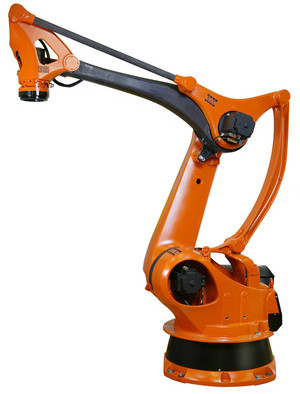
\includegraphics[width=.65\linewidth]{fig_01}
%\textit{}
\end{center}
\begin{obj}
Objectif : Dans cette étude, on va mettre en évidence l’influence du frottement sur l’équilibre d’un système.
\end{obj}

On note  $\vect{P_3}$ le poids de la charge appliquée sur le coulisseau et $\vect{F_m}$ l’effort appliqué en $E$ par l’opérateur sur le levier à excentrique \textbf{(1)}.

\subsection*{Paramétrage géométrique}
$\vect{AB}=L_0\vect{x_0}$; 
$\vect{AE}=-L_1\vect{x_1}$; 
$\vect{BI}=d_0\vect{x_0}$; 
$\vect{AC}=e_1\vect{x_1}$; 
$\vect{HC}=R_1\vect{y_2}$; 
$\vect{BJ}=\lambda_{32}\vect{x_2}$; 
$\vect{ID}=\lambda_{30}\vect{y_0}$; 
$\vect{JD}=R_3\vect{y_2}$; 
$\left(\vect{x_0},\vect{x_1} \right)=\theta_{\left(1/0\right)}$; 
$\left(\vect{x_0},\vect{x_2} \right)=\theta_{\left(2/0\right)}$.
 	 	 	 	 

\subsection*{On suppose dans un premier temps que toutes les liaisons sont sans frottement.}
\question{Justifier que le système est statiquement plan.}
\question{En écrivant les équations associées à l’équilibre de chacune des pièces, établir la relation liant $F_m$ et $P_3$ à l’équilibre.   \textit{On cherchera à écrire le minimum d'équations.}}
%\question{Indiquer quelles sont les équations qui auraient pu permettre de trouver cette relation sans écrire tout le système d’équation.}
\question{Pour quelle(s) valeur(s) particulières de $\theta_{1/0}$ l’équilibre est-il possible avec un effort $F_m$ nul ?}
\question{Établir les équations permettant de relier la translation $\lambda_{3/0}$ du coulisseau, la position angulaire $\theta_{(1/0)}$ et les constantes géométriques du mécanisme.}
\question{En établissant un bilan de puissance, vérifier les relations obtenues.}

\subsection*{On suppose que les contacts en $H$ et $J$ s’effectuent avec frottement de même coefficient $f$}

\question{On suppose que les contacts en $H$ et $J$ s’effectuent avec frottement de même coefficient $f$. Reprendre la question 2 dans le cadre de cette hypothèse. On se place dans la situation de descente de la charge.}

Distinguer deux situations, selon que $J$ est situé au-dessus ou en dessous de l’axe $\left(B,\vect{x_0}\right)$.
\question{Définir le domaine de valeurs de $\theta_{(1/0)}$ pour lequel l’équilibre du système est possible sans exercer d’effort sur le levier \textbf{(1)} ($F_m = 0$)}.

